
\section{1A2 MOE Models}

\begin{table}[H]
\caption{1A2 MOE Model Results}
\begin{minipage}{.5\linewidth}
\centering
\begin{tabular}{|l|l|l|l|}
\hline
\multicolumn{4}{|c|}{1A2 Training Set Accuracy}   \\ \hline
PC & Total          & Active          & Inactive  \\ \hline
2  & 0.638          & 0.752           & 0.522     \\ \hline
5  & 0.704          & 0.746           & 0.662     \\ \hline
10 & 0.734          & 0.755           & 0.712     \\ \hline
15 & 0.737          & 0.770           & 0.704     \\ \hline
20 & 0.741          & 0.781           & 0.701     \\ \hline
30 & 0.735          & 0.782           & 0.686     \\ \hline
44 & 0.725          & 0.777           & 0.672     \\ \hline
\end{tabular}
\end{minipage}
\begin{minipage}{.5\linewidth}
\centering
\begin{tabular}{|l|l|l|l|}
\hline
\multicolumn{4}{|c|}{1A2 Test Set Accuracy}     \\ \hline
PC & Total          & Active          & Inactive \\ \hline
2  & 0.632          & 0.758           & 0.517   \\ \hline
5  & 0.705          & 0.773           & 0.643   \\ \hline
10 & 0.746          & 0.749           & 0.743   \\ \hline
15 & 0.752          & 0.775           & 0.731   \\ \hline
20 & 0.748          & 0.779           & 0.721   \\ \hline
30 & 0.739          & 0.783           & 0.698   \\ \hline
44 & 0.720          & 0.773           & 0.672   \\ \hline
\end{tabular}
\end{minipage}
\end{table}

Cytochrome P450 isozyme 1A2 models were trained on 4820 actives and 4780 inactives in the training set, and validated against 529 actives and 580 inactives in the test set. All models are considered good models when the total accuracy is above 0.6. The test set results represent compounds unseen by the model. Validating these models against the test set does not produce wildly divergent accuracy scores, indicating that overfitting is unlikely. 

\begin{figure}[H]
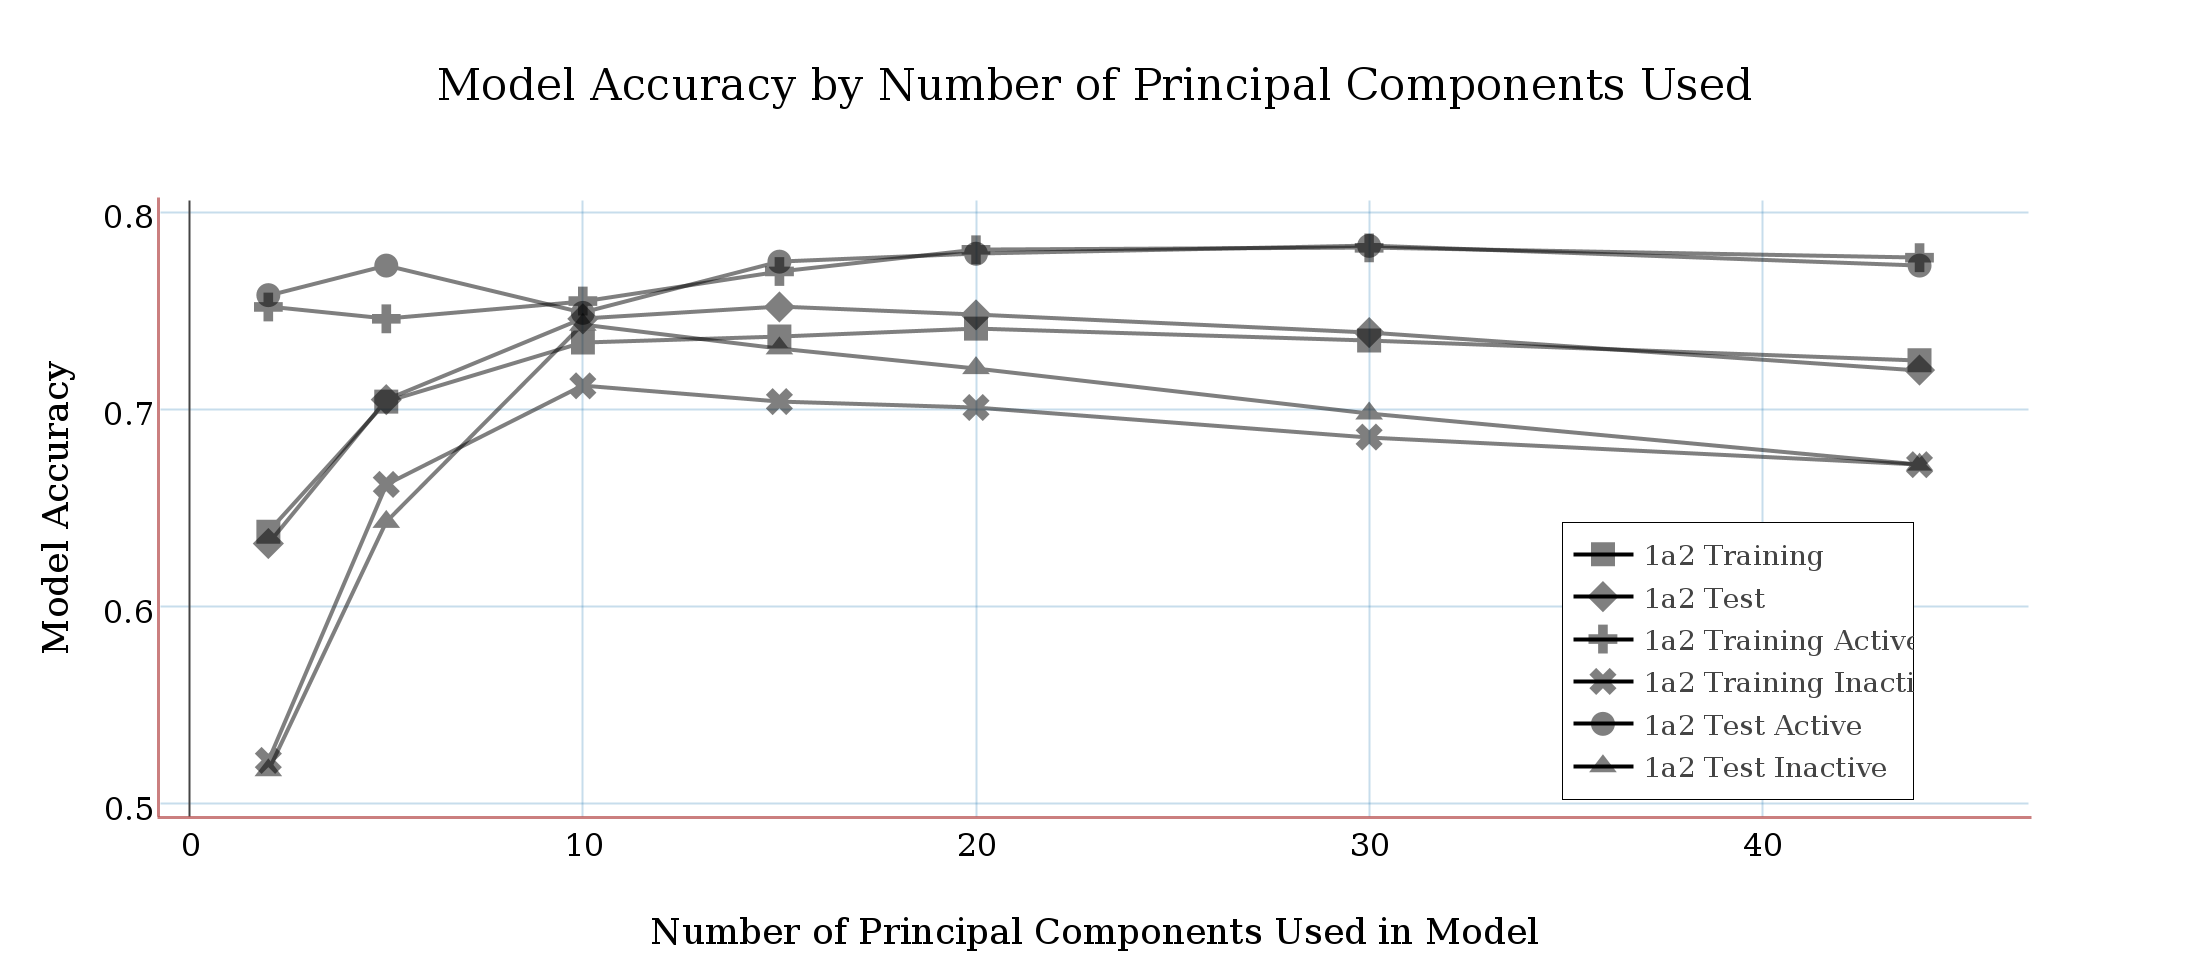
\includegraphics[width=1\textwidth]{../img/1a2_moe_model_accuracy.png}
\caption{1A2 MOE Model Accuracy}
\label{fig:1a2}
\end{figure}

A visual scan of Figure \ref{fig:1a2} shows that model accuracy is higher for predicting active compounds than inactive compounds, and total accuracy is somewhere in between. 20 pricipal components (PC20) appears to be an optimal number for capturing relevant variance.
PC20 is approximately the point at which total accuracy is maximized and dropoff of accuracy on inactives at either end of the range is avoided.
At 20PCs, the total accuracy on the test set is 0.748. Accuracy on Actives is 0.779 and accuracy on inactives is 0.721.


\section{2C9 MOE Models}

\begin{table}[H]
\caption{2C9 MOE Model Results}
\begin{minipage}{.5\linewidth}
\centering
\begin{tabular}{|l|l|l|l|}
\hline
\multicolumn{4}{|c|}{2C9 Training Set Accuracy} \\ \hline
PC & Total          & Active          & Inactive\\ \hline
2  & 0.620          & 0.695           & 0.547   \\ \hline
5  & 0.683          & 0.722           & 0.645   \\ \hline
10 & 0.699          & 0.744           & 0.655   \\ \hline
15 & 0.702          & 0.752           & 0.653   \\ \hline
20 & 0.710          & 0.756           & 0.665   \\ \hline
30 & 0.711          & 0.754           & 0.668   \\ \hline
44 & 0.712          & 0.770           & 0.655   \\ \hline
\end{tabular}
\end{minipage}
\begin{minipage}{.5\linewidth}
\centering
\begin{tabular}{|l|l|l|l|}
\hline
\multicolumn{4}{|c|}{2C9 Test Set Accuracy}     \\ \hline
PC & Total          & Active          & Inactive\\ \hline
2  & 0.609          & 0.702           & 0.510   \\ \hline
5  & 0.675          & 0.713           & 0.634   \\ \hline
10 & 0.682          & 0.730           & 0.632   \\ \hline
15 & 0.686          & 0.739           & 0.630   \\ \hline
20 & 0.685          & 0.731           & 0.636   \\ \hline
30 & 0.690          & 0.730           & 0.646   \\ \hline
44 & 0.688          & 0.750           & 0.621   \\ \hline
\end{tabular}
\end{minipage}
\end{table}

Cytochrome P450 isozyme 2C9 models were trained on 3266 actives and 3327 inactives in the training set, and validated against 855 actives and 794 inactives in the test set. All models are considered good models when the total accuracy is above 0.6. The test set results represent compounds unseen by the model. Validating these models against the test set does not produce wildly divergent accuracy scores, indicating that overfitting is unlikely.

\begin{figure}[H]
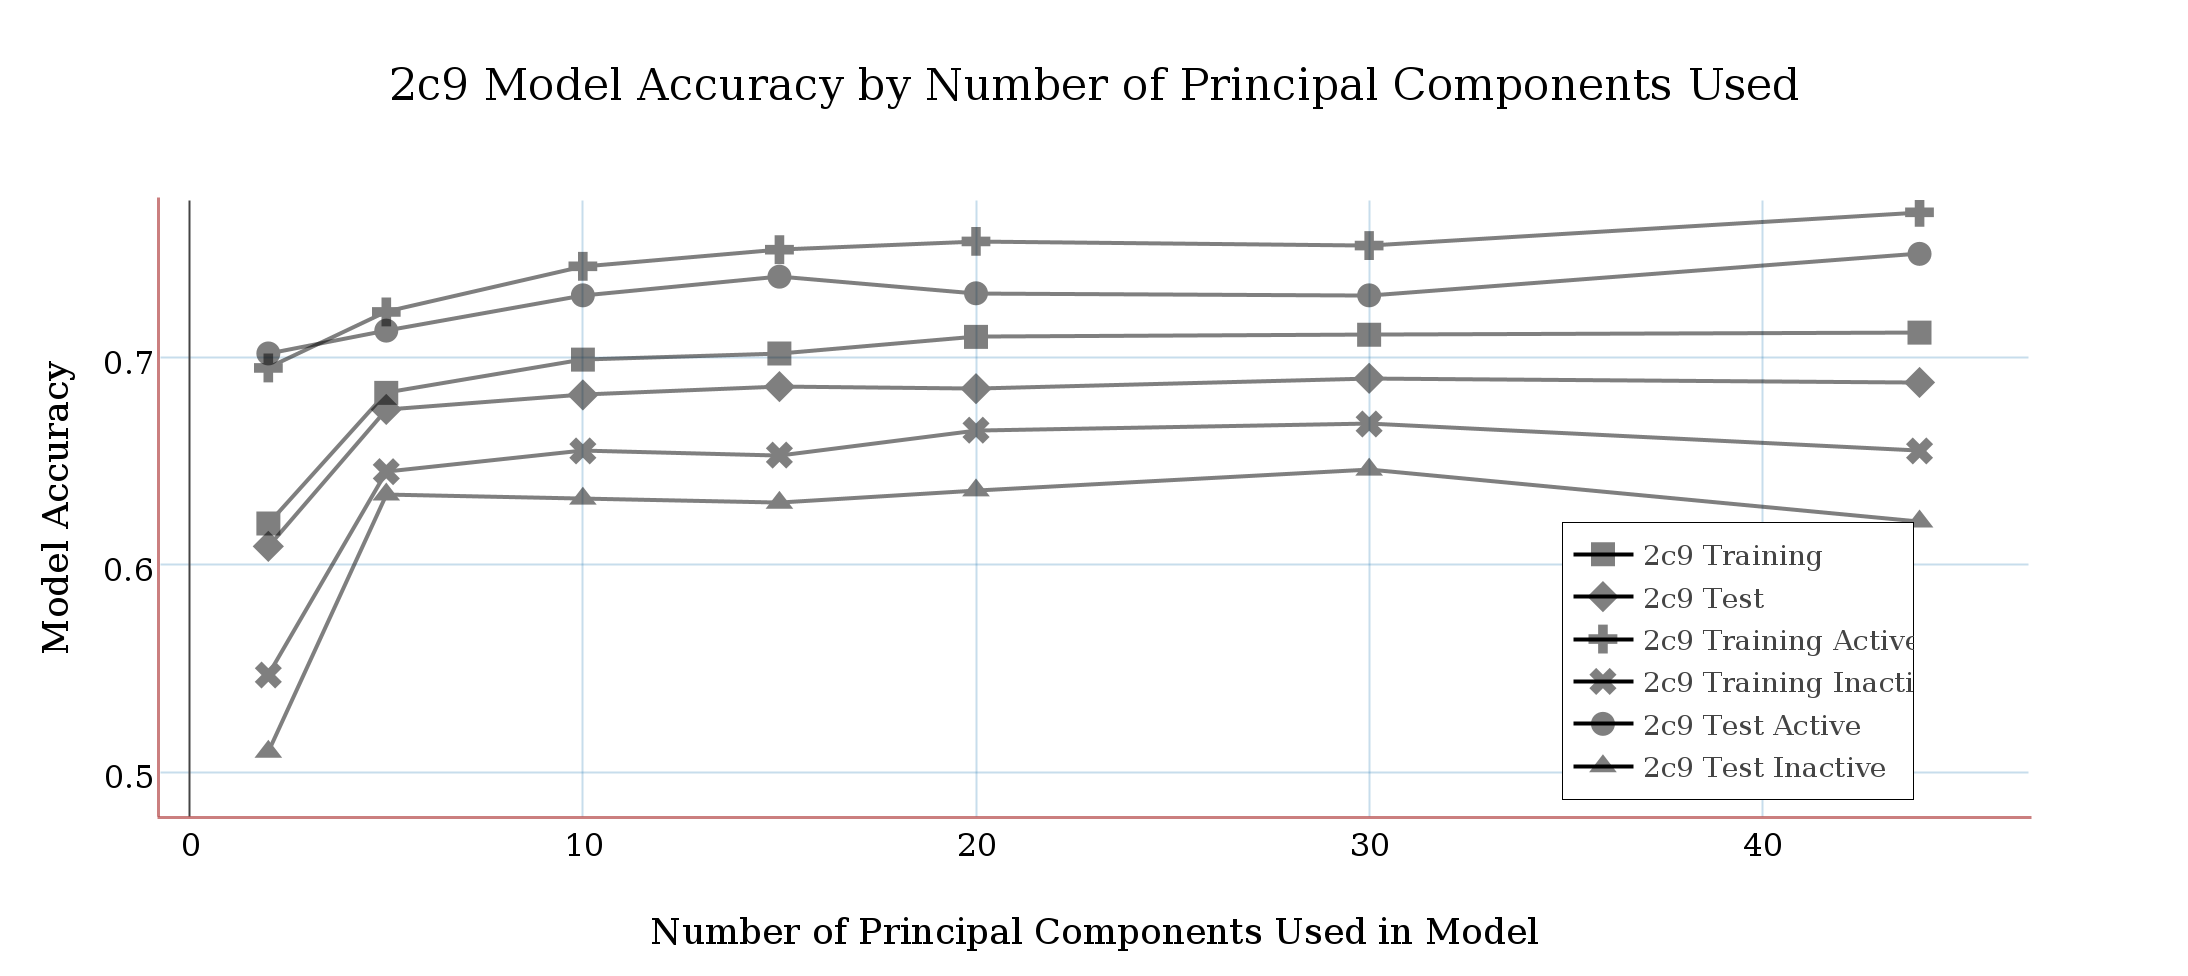
\includegraphics[width=1\textwidth]{../img/2c9_moe_model_accuracy.png}
\caption{2C19 MOE Model Accuracy}
\label{fig:2c9}
\end{figure}

A visual scan of Figure \ref{fig:2c9} shows that model accuracy is higher for predicting active compounds than inactive compounds, and total accuracy is somewhere in between. 20 pricipal components appears to be an optimal number for capturing relevant variance.
PC20 is approximately the point at which total accuracy is maximized and dropoff of accuracy on inactives at either end of the range is avoided.
At 20PCs, the total accuracy on the test set is 0.685. Accuracy on Actives is 0.731 and accuracy on inactives is 0.636.


\section{2C19 MOE models}

\begin{table}[H]
\caption{2C19 MOE Model Results}
\begin{minipage}{.5\linewidth}
\centering
\begin{tabular}{|l|l|l|l|}
\hline
\multicolumn{4}{|c|}{2C19 Training Set Accuracy} \\ \hline
PC & Total          & Active          & Inactive \\ \hline
2  & 0.585          & 0.774           & 0.396   \\ \hline
5  & 0.685          & 0.726           & 0.645   \\ \hline
10 & 0.699          & 0.736           & 0.661    \\ \hline
15 & 0.700          & 0.747           & 0.653    \\ \hline
20 & 0.705          & 0.749           & 0.661    \\ \hline
30 & 0.717          & 0.761           & 0.672    \\ \hline
44 & 0.708          & 0.777           & 0.640    \\ \hline
\end{tabular}
\end{minipage}%
\begin{minipage}{.5\linewidth}
\centering
\begin{tabular}{|l|l|l|l|}
\hline
\multicolumn{4}{|c|}{2C19 Test Set Accuracy}       \\ \hline
PC & Total          & Active          & Inactive   \\ \hline
2  & 0.593          & 0.775           & 0.408      \\ \hline
5  & 0.683          & 0.729           & 0.635      \\ \hline
10 & 0.691          & 0.731           & 0.650      \\ \hline
15 & 0.687          & 0.736           & 0.637      \\ \hline
20 & 0.698          & 0.758           & 0.638      \\ \hline
30 & 0.699          & 0.764           & 0.633      \\ \hline
44 & 0.694          & 0.774           & 0.613      \\ \hline
\end{tabular}
\end{minipage}
\end{table}

Cytochrome P450 isozyme 2C19 models were trained on 4721 actives and 4741 inactives in the training set, and validated against 1193 actives and 1173 inactives in the test set. All models are considered good models when the  total accuracy is above 0.6.  The test set results represent compounds unseen by the model. Validating these models against the test set does not produce wildly divergent accuracy scores, indicating that overfitting is unlikely. 


\begin{figure}[H]
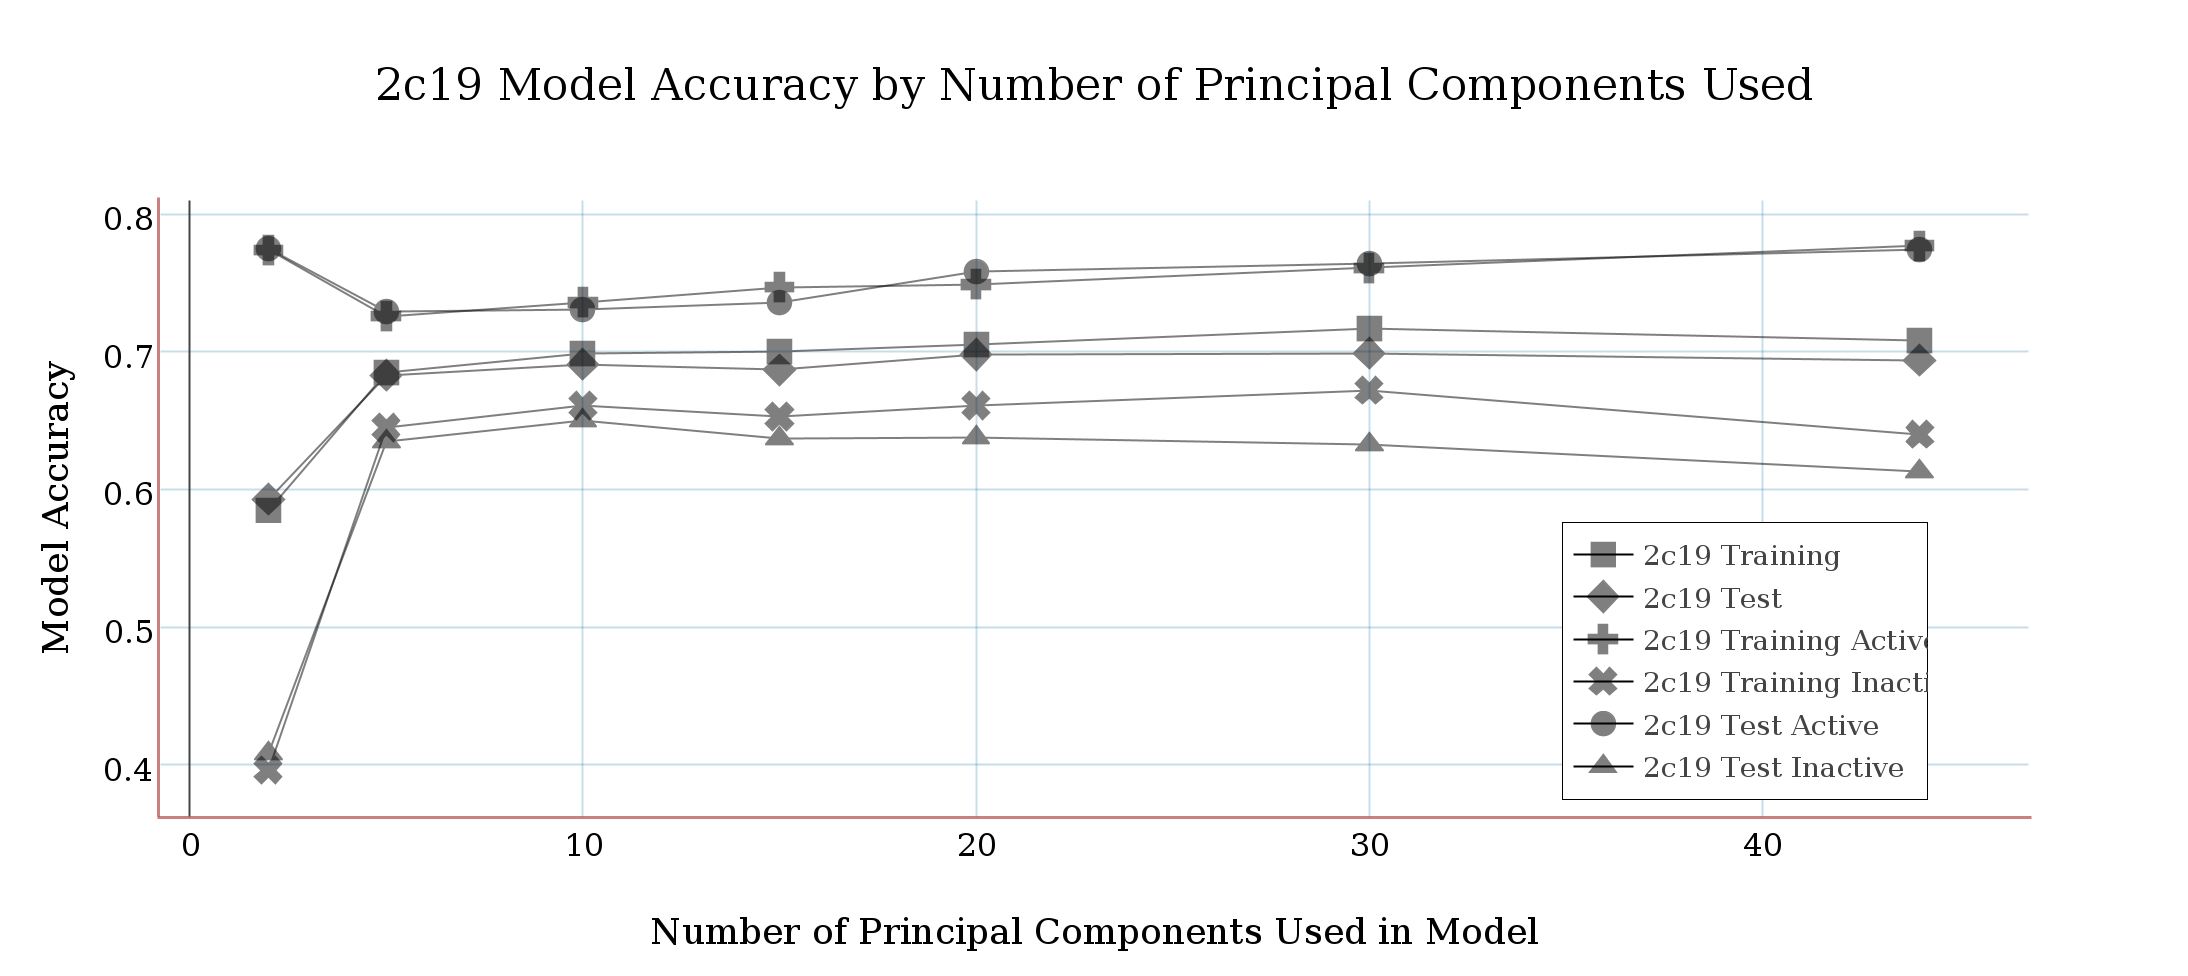
\includegraphics[width=1\textwidth]{../img/2c19_moe_model_accuracy.png}
\caption{2C19 MOE Model Accuracy}
\label{fig:2c19}
\end{figure}

A visual scan of Figure \ref{fig:2c19} shows that model accuracy is higher for predicting active compounds than inactive compounds, and total accuracy is somewhere in between. 20 pricipal components appears to be an optimal number for capturing relevant variance.
PC20 is approximately the point at which total accuracy is maximized and dropoff of accuracy on inactives at either end of the range is avoided.
At 20PCs, the total accuracy on the test set is 0.698. Accuracy on Actives is 0.758 and accuracy on inactives is 0.638.


\section{2D6 MOE Models}

\begin{table}[H]
\caption{2D6 MOE Model Results}
\begin{minipage}{.5\linewidth}
\centering
\begin{tabular}{|l|l|l|l|}
\hline
\multicolumn{4}{|c|}{2D6 Training Set Accuracy} \\ \hline
PC & Total          & Active          & Inactive\\ \hline
2  & 0.589          & 0.753           & 0.426   \\ \hline
5  & 0.670          & 0.706           & 0.634   \\ \hline
10 & 0.685          & 0.721           & 0.648   \\ \hline
15 & 0.686          & 0.709           & 0.662   \\ \hline
20 & 0.705          & 0.721           & 0.689   \\ \hline
30 & 0.703          & 0.732           & 0.673   \\ \hline
44 & 0.690          & 0.725           & 0.656   \\ \hline
\end{tabular}
\end{minipage}
\begin{minipage}{.5\linewidth}
\centering
\begin{tabular}{|l|l|l|l|}
\hline
\multicolumn{4}{|c|}{2D6 Test Set Accuracy}      \\ \hline
PC & Total          & Active          & Inactive \\ \hline
2  & 0.590          & 0.738           & 0.443    \\ \hline
5  & 0.667          & 0.685           & 0.650    \\ \hline
10 & 0.662          & 0.688           & 0.636    \\ \hline
15 & 0.665          & 0.692           & 0.639    \\ \hline
20 & 0.683          & 0.699           & 0.668    \\ \hline
30 & 0.686          & 0.696           & 0.677    \\ \hline
44 & 0.669          & 0.707           & 0.632    \\ \hline
\end{tabular}
\end{minipage}
\end{table}

Cytochrome P450 isozyme 2D6 models were trained on 2219 of actives and 2214 of inactives in the training set, and validated against 552 actives and 557 inactives in the test set. All models are considered good models when the total accuracy is above 0.6. The test set results represent compounds unseen by the model. Validating these models against the test set does not produce wildly divergent accuracy scores, indicating that overfitting is unlikely.

\begin{figure}[H]
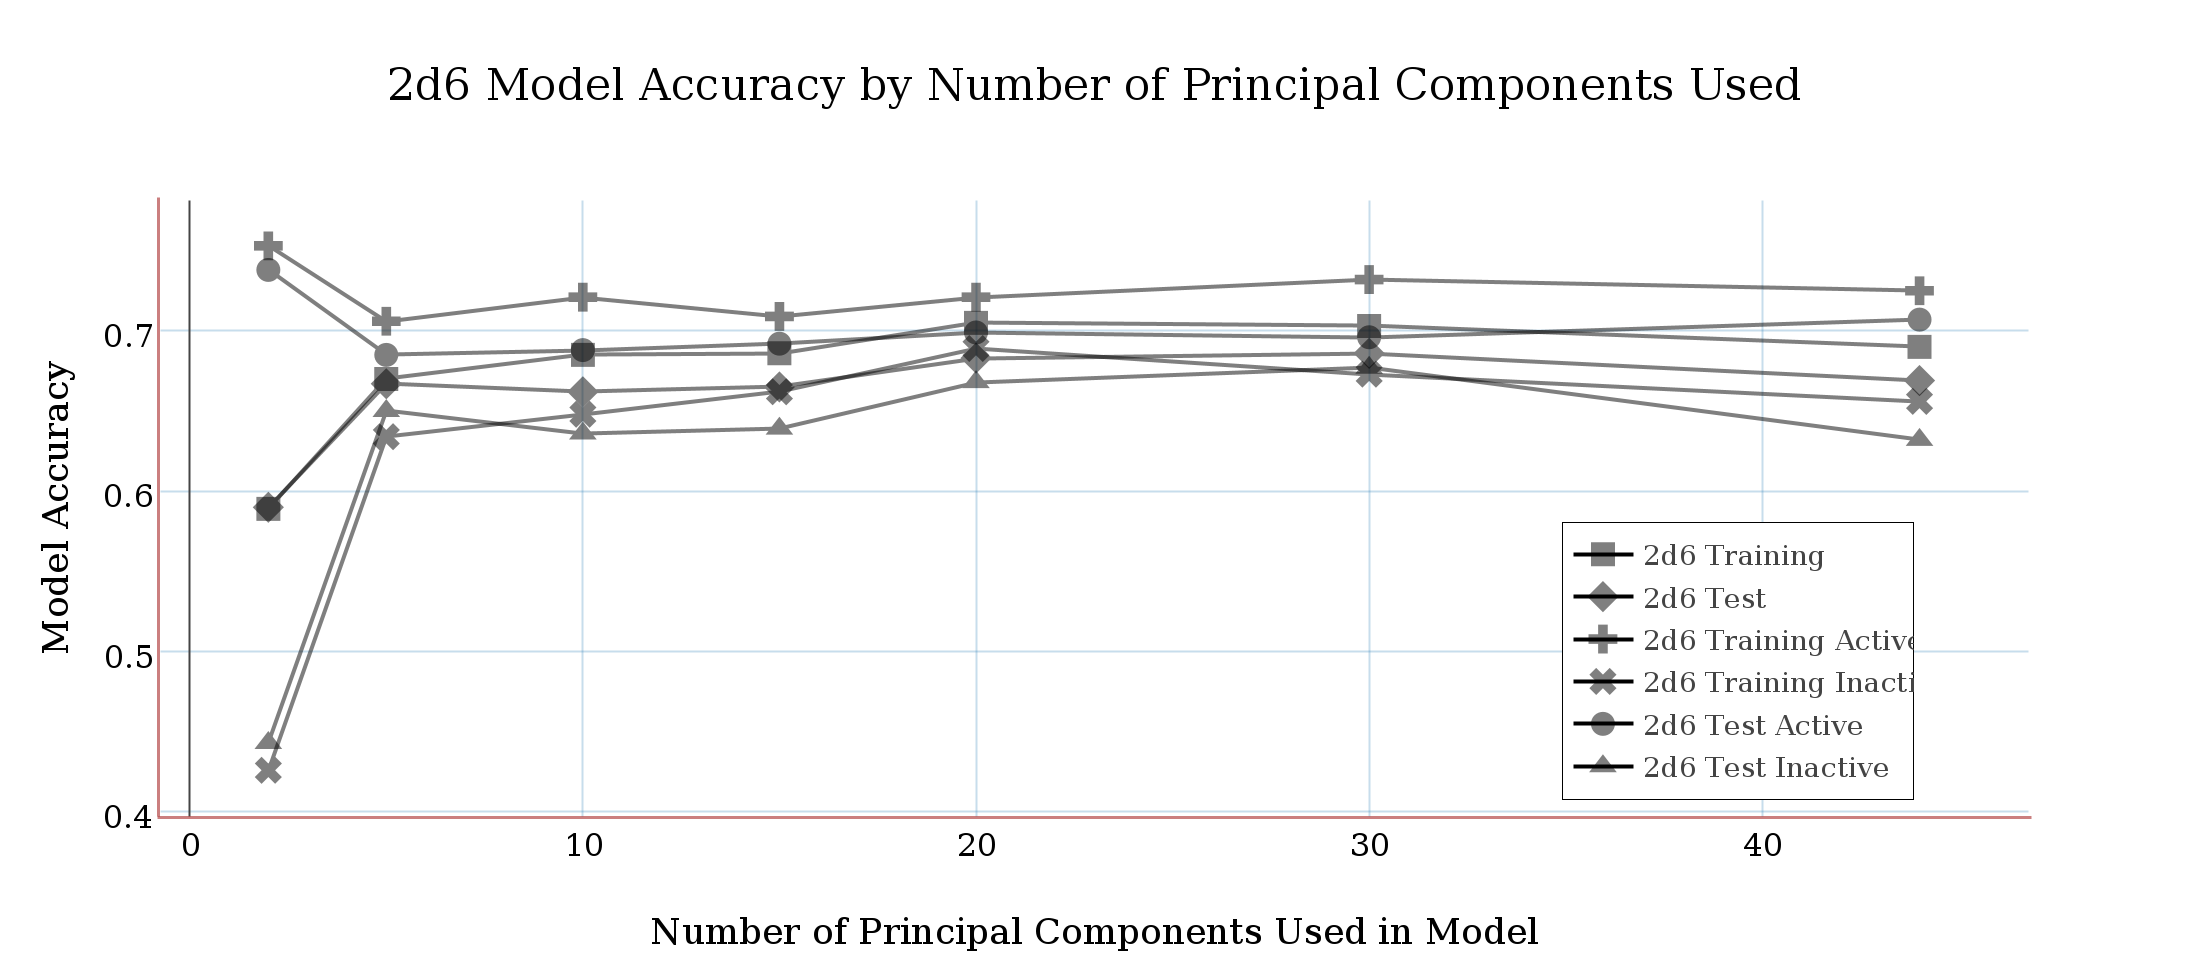
\includegraphics[width=1\textwidth]{../img/2d6_moe_model_accuracy.png}
\caption{2D6 MOE Model Accuracy}
\label{fig:2d6}
\end{figure}

A visual scan of Figure \ref{fig:2d6} shows that model accuracy is higher for predicting active compounds than inactive compounds, and total accuracy is somewhere in between. 20 pricipal components appears to be an optimal number for capturing relevant variance.
PC20 is approximately the point at which total accuracy is maximized and dropoff of accuracy on inactives at either end of the range is avoided.
At 20PCs, the total accuracy on the test set is 0.683. Accuracy on Actives is 0.699 and accuracy on inactives is 0.668.


\section{3A4 MOE Models}

\begin{table}[H]
\caption{3A4 MOE Model Results}
\begin{minipage}{.5\linewidth}
\centering
\begin{tabular}{|l|l|l|l|}
\hline
\multicolumn{4}{|c|}{3A4 Training Set Accuracy} \\ \hline
PC & Total          & Active          & Inactive \\ \hline
2  & 0.644          & 0.699           & 0.589   \\ \hline
5  & 0.675          & 0.727           & 0.623   \\ \hline
10 & 0.698          & 0.741           & 0.655   \\ \hline
15 & 0.701          & 0.746           & 0.656   \\ \hline
20 & 0.705          & 0.749           & 0.660   \\ \hline
30 & 0.709          & 0.761           & 0.657   \\ \hline
44 & 0.698          & 0.773           & 0.623   \\ \hline
\end{tabular}
\end{minipage}
\begin{minipage}{.5\linewidth}
\centering
\begin{tabular}{|l|l|l|l|}
\hline
\multicolumn{4}{|c|}{3A4 Test Set Accuracy}      \\ \hline
PC & Total          & Active          & Inactive \\ \hline
2  & 0.627          & 0.683           & 0.573    \\ \hline
5  & 0.656          & 0.719           & 0.595    \\ \hline
10 & 0.677          & 0.719           & 0.637    \\ \hline
15 & 0.680          & 0.733           & 0.628    \\ \hline
20 & 0.686          & 0.736           & 0.638    \\ \hline
30 & 0.686          & 0.742           & 0.631    \\ \hline
44 & 0.676          & 0.747           & 0.607    \\ \hline
\end{tabular}
\end{minipage}
\end{table}

Cytochrome P450 isozyme 3A4 models were trained on 4234 of actives and 4193 of inactives in the training set, and validated against 1033 actives and 1074 inactives in the test set. All models are considered good models when the total accuracy is above 0.6. The test set results represent compounds unseen by the model. Validating these models against the test set does not produce wildly divergent accuracy scores, indicating that overfitting is unlikely.

\begin{figure}[H]
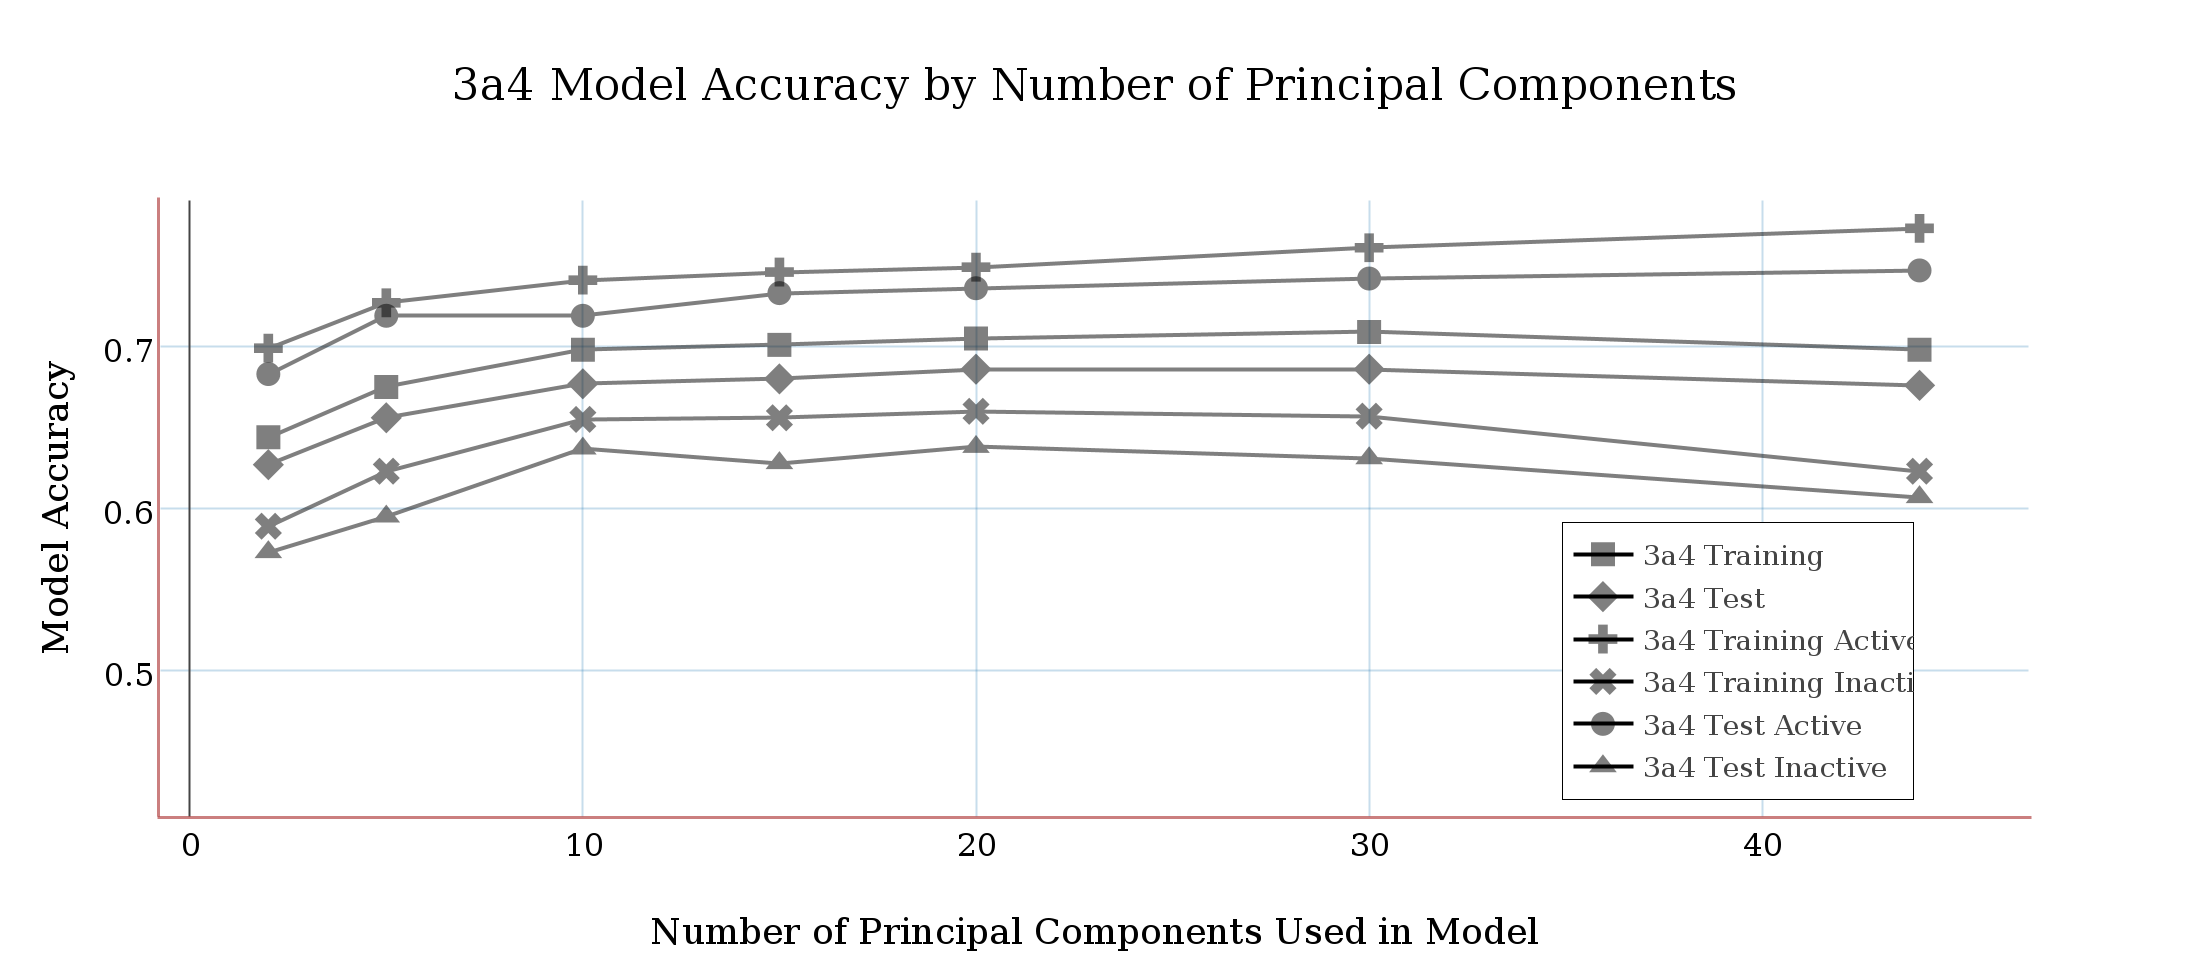
\includegraphics[width=1\textwidth]{../img/3a4_moe_model_accuracy.png}
\caption{3A4 MOE Model Accuracy}
\label{fig:3a4}
\end{figure}

A visual scan of Figure \ref{fig:3a4} shows that model accuracy is higher for predicting active compounds than inactive compounds, and total accuracy is somewhere in between. 20 pricipal components appears to be an optimal number for capturing relevant variance.
PC20 is approximately the point at which total accuracy is maximized and dropoff of accuracy on inactives at either end of the range is avoided.
At 20PCs, the total accuracy on the test set is 0.686. Accuracy on Actives is 0.736 and accuracy on inactives is 0.638.


\section{1A2 Classification Method Comparison}

\begin{table}[H]
\caption{Comparison of Classification Methods for 1A2}
\centering
\begin{tabular}{|l|l|l|}
\hline
\multicolumn{3}{|c|}{1A2 Classification Method Comparison} \\ \hline
          & Training Set & Test Set \\ \hline
MOE 20PC  & 0.741        & 0.748    \\ \hline
kNN       & 0.761        & 0.754    \\ \hline
Random Forest & 0.770    & 0.769    \\ \hline
SVM       & 0.800        & 0.804    \\ \hline
\end{tabular}
\end{table}

The comparison of model accuracy results on the CYP 1A2 isozyme dataset show that Binary QSAR implemented in the Molecular Operating Environment gave an overall accuracy of 0.748 for the test set, while the methods implemented by Python's scikit-learn gave accuracies of 0.754 for k-nearest neighbor, 0.769 for random forests and 0.804 for support vector machines on the test set.

\section{2C9 Classification Method Comparison}

\begin{table}[H]
\caption{Comparison of Classification Methods for 2C9}
\centering
\begin{tabular}{|l|l|l|}
\hline
\multicolumn{3}{|c|}{2C9 Classification Method Comparison} \\ \hline
          & Training Set & Test Set \\ \hline
MOE 20PC  & 0.710        & 0.685    \\ \hline
kNN       & 0.721        & 0.692    \\ \hline
Random Forest & 0.717    & 0.687    \\ \hline
SVM       & 0.749        & 0.720    \\ \hline
\end{tabular}
\end{table}

The comparison of model accuracy results on the CYP 2C9 isozyme dataset show that Binary QSAR implemented in the Molecular Operating Environment gave an overall accuracy of 0.685 for the test set, while the methods implemented by Python's scikit-learn gave accuracies of 0.692 for k-nearest neighbor, 0.687 for random forests and 0.720 for support vector machines on the test set.

\section{2C19 Classification Method Comparison}

\begin{table}[H]
\caption{Comparison of Classification Methods for 2C19}
\centering
\begin{tabular}{|l|l|l|}
\hline
\multicolumn{3}{|c|}{2C19 Classification Method Comparison} \\ \hline
          & Training Set & Test Set \\ \hline
MOE 20PC  & 0.705        & 0.698    \\ \hline
kNN       & 0.730        & 0.720    \\ \hline
Random Forest & 0.736    & 0.721    \\ \hline
SVM       & 0.767        & 0.756    \\ \hline
\end{tabular}
\end{table}

The comparison of model accuracy results on the CYP 2C19 isozyme dataset show that Binary QSAR implemented in the Molecular Operating Environment gave an overall accuracy of 0.698 for the test set, while the methods implemented by Python's scikit-learn gave accuracies of 0.720 for k-nearest neighbor, 0.721 for random forests and 0.756 for support vector machines on the test set.

\section{2D6 Classification Method Comparison}

\begin{table}[H]
\caption{Comparison of Classification Methods for 2D6}
\centering
\begin{tabular}{|l|l|l|}
\hline
\multicolumn{3}{|c|}{2D6 Classification Method Comparison} \\ \hline
          & Training Set & Test Set \\ \hline
MOE 20PC  & 0.705        & 0.683    \\ \hline
kNN       & 0.717        & 0.678    \\ \hline
Random Forest & 0.729    & 0.707    \\ \hline
SVM       & 0.755        & 0.725    \\ \hline
\end{tabular}
\end{table}

The comparison of model accuracy results on the CYP 2D6 isozyme dataset show that Binary QSAR implemented in the Molecular Operating Environment gave an overall accuracy of 0.683 for the test set, while the methods implemented by Python's scikit-learn gave accuracies of 0.678 for k-nearest neighbor, 0.707 for random forests and 0.725 for support vector machines on the test set.


\section{3A4 Classification Method Comparison}

\begin{table}[H]
\caption{Comparison of Classification Methods for 3A4}
\centering
\begin{tabular}{|l|l|l|}
\hline
\multicolumn{3}{|c|}{3A4 Classification Method Comparison} \\ \hline
          & Training Set & Test Set \\ \hline
MOE 20PC  & 0.705        & 0.686    \\ \hline
kNN       & 0.716        & 0.674    \\ \hline
Random Forest & 0.719    & 0.683    \\ \hline
SVM       & 0.755        & 0.714    \\ \hline
\end{tabular}
\end{table}

The comparison of model accuracy results on the CYP 3A4 isozyme dataset show that Binary QSAR implemented in the Molecular Operating Environment gave an overall accuracy of 0.686 for the test set, while the methods implemented by Python's scikit-learn gave accuracies of 0.674 for k-nearest neighbor, 0.683 for random forests and 0.714 for support vector machines on the test set.


\section{Overall Method Comparison}

\begin{figure}[H]
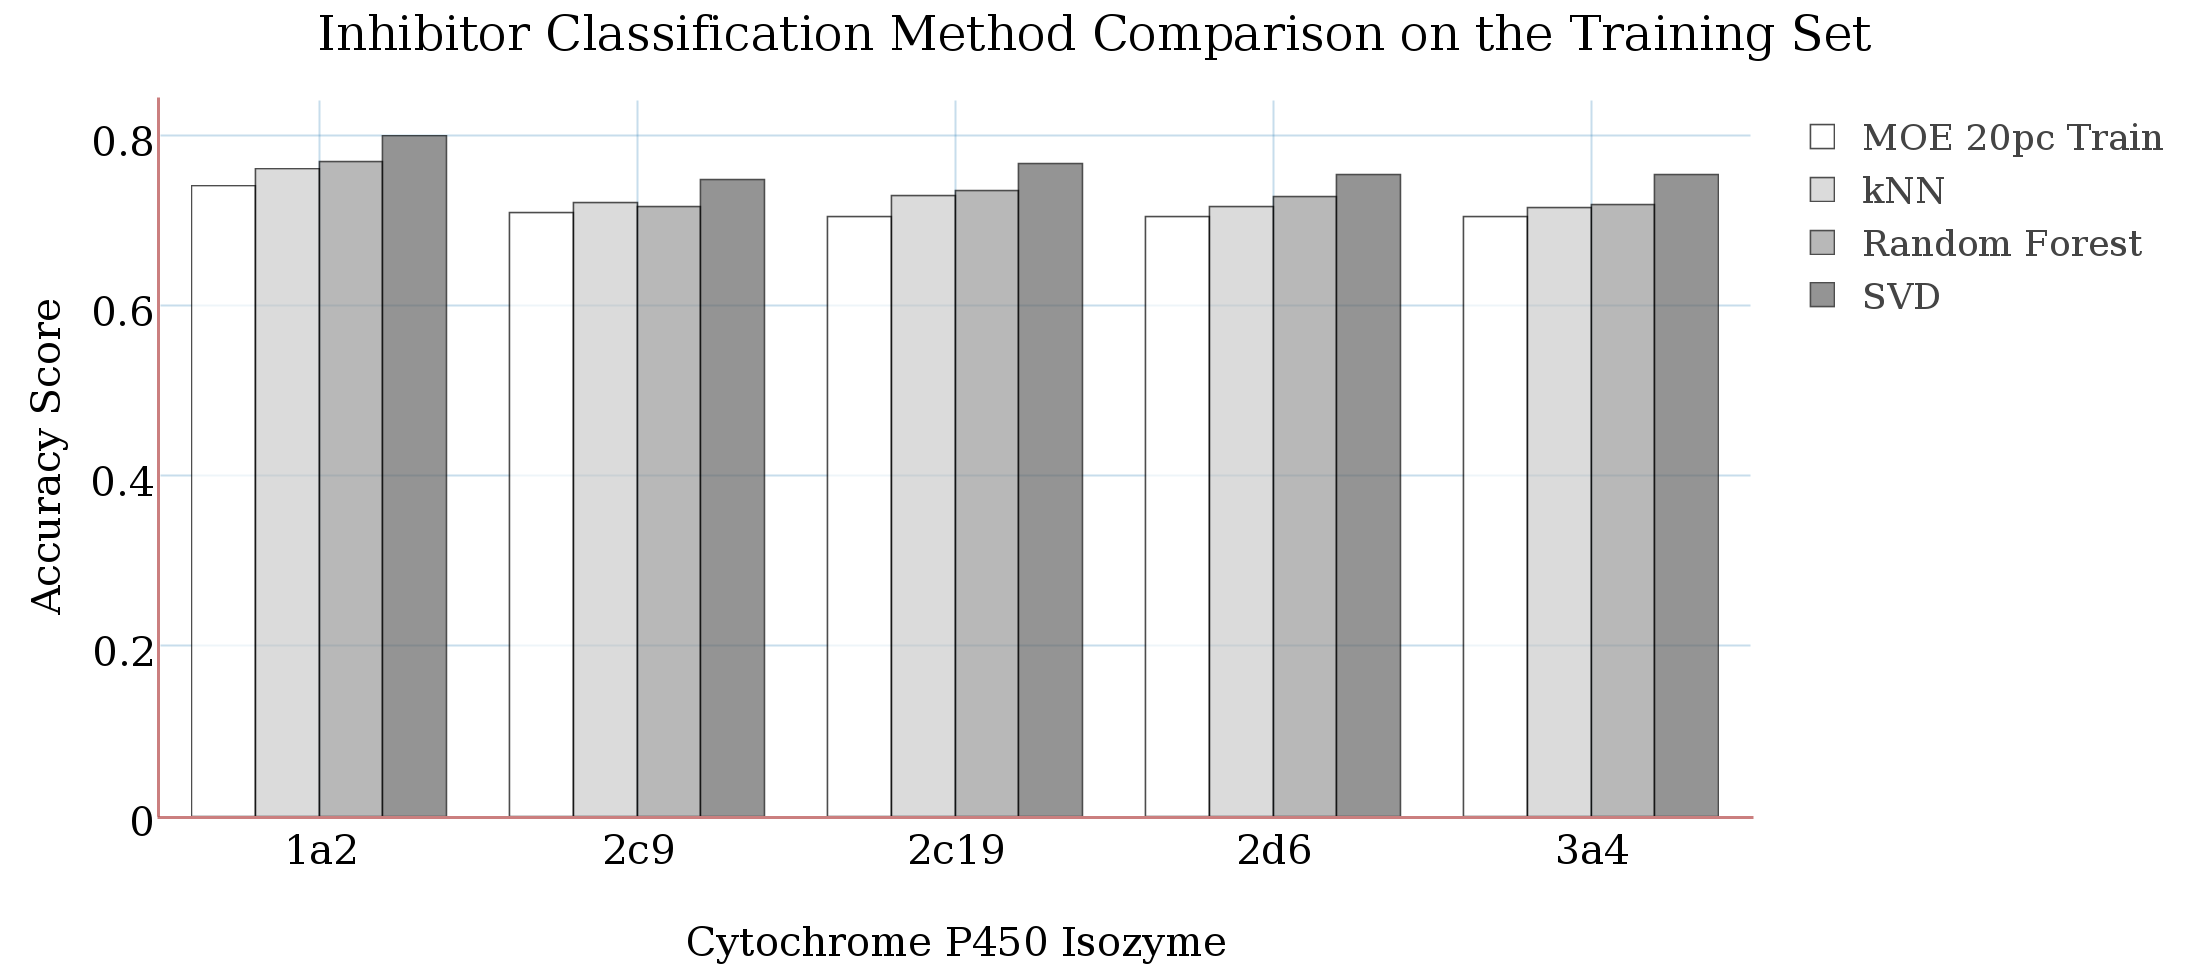
\includegraphics[width=1\textwidth]{../img/method_comparison_training_set.png}
\caption{Inhibitor Classification Method Comparison on the Training Set}
\end{figure}

Looking at the results for method comparison on the test set, it is clear that all methods performed similarly for each isozyme and well overall. It appears that the support vector machine classifier slightly outperforms all others in each case.

\begin{figure}[H]
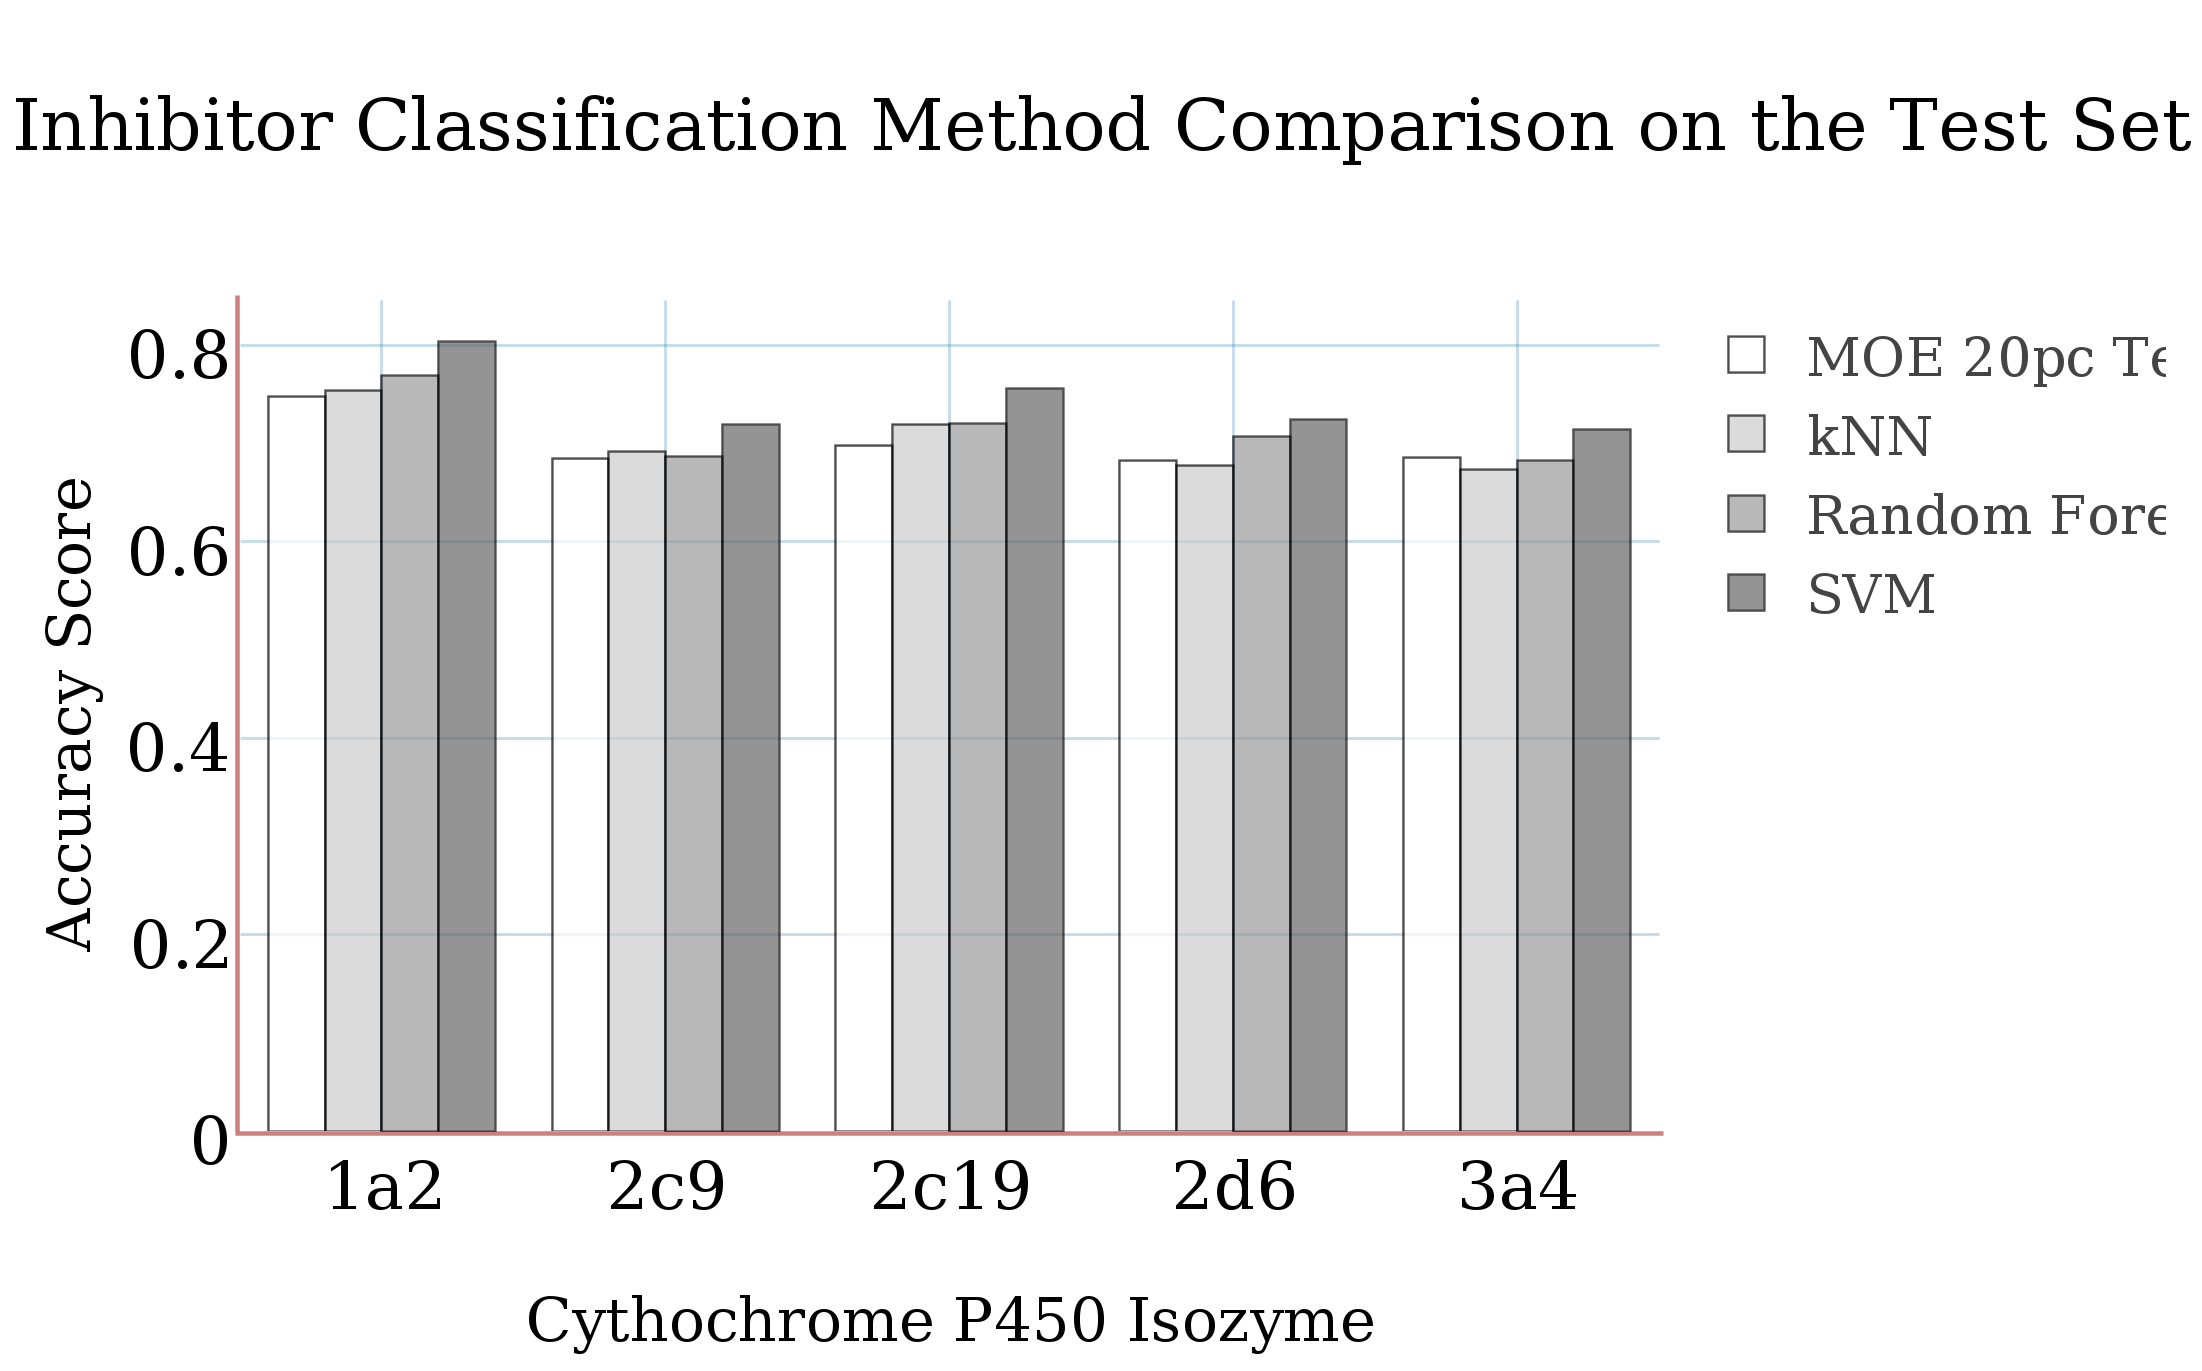
\includegraphics[width=1\textwidth]{../img/method_comparison_test_set.png}
\caption{Inhibitor Classification Method Comparison on the Test Set}
\end{figure}

Looking at the results for method comparison on the test set, it is clear that all methods performed similarly for each isozyme and well overall. It appears that the support vector machine classifier slightly outperforms all others in each case.




